\chapter{ADM-ARCHIMATE}
\section{Introducción}
\newpage

\section{ADM}

\begin{figure}[th!]
	\centering
	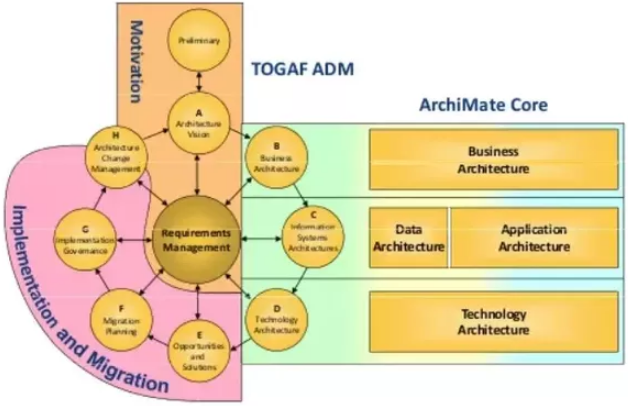
\includegraphics[width=0.7\linewidth]{arquitectura/adm_lenguaje/imgs/adm}
	\caption{ADM}
	\label{fig:adm}
\end{figure}

\newpage

\subsection{Glosario Conceptos Capa de Negocio}

\begin{longtable}[c]{|p{2.5cm}|l|c|}
	\caption{Conceptos Capa de Negocio}
	\label{my-label}\\
	\hline
	\textbf{Concepto} 			& \textbf{Descripción}                                                                                                                                            & \textbf{Notación} \\ \hline
	\endhead
	%
	Actor de Negocio  			& \begin{tabular}[c]{p{7cm}@{}l@{}}Entidad organizacional que es capaz de comportamiento de ejecución\end{tabular}                                                    & 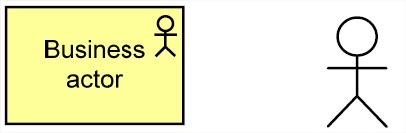
\includegraphics[width=35mm]{arquitectura/adm_lenguaje/imgs/business/BusinessActor}           \\ \hline
	Rol de Negocio    			& \begin{tabular}[c]{p{7cm}@{}l@{}}Responsabilidad de realizar acciones específicas según su comportamiento, ante el cual un actor puede ser asignado\end{tabular} & 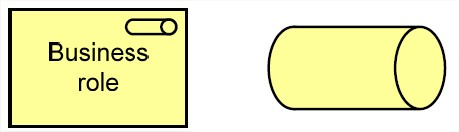
\includegraphics[width=35mm]{arquitectura/adm_lenguaje/imgs/business/BusinessRole}          \\ \hline
	Colaboración de Negocio  	& \begin{tabular}[c]{p{7cm}@{}l@{}}Agregado de dos o más roles de negocio que trabajan juntos para realizar comportamiento colectivo.\end{tabular} & 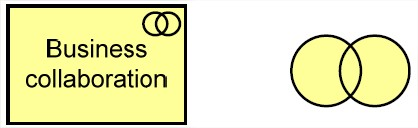
\includegraphics[width=35mm]{arquitectura/adm_lenguaje/imgs/business/BusinessCollaboration}          \\ \hline
	Interfaz de Negocio    		& \begin{tabular}[c]{p{7cm}@{}l@{}}Un punto de acceso donde un servicio comercial está disponible para el medio ambiente.\end{tabular} & 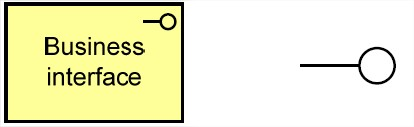
\includegraphics[width=35mm]{arquitectura/adm_lenguaje/imgs/business/BusinessInterface}          \\ \hline
	Localización    			& \begin{tabular}[c]{p{7cm}@{}l@{}}Un punto o extensión conceptual en el espacio.\end{tabular} & 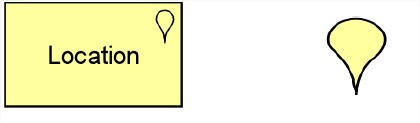
\includegraphics[width=35mm]{arquitectura/adm_lenguaje/imgs/business/Location}          \\ \hline
	Objeto de Negocio    		& \begin{tabular}[c]{p{7cm}@{}l@{}}Un elemento pasivo que tiene relevancia de una perspectiva comercial.\end{tabular} & 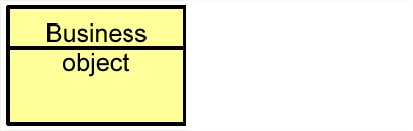
\includegraphics[width=35mm]{arquitectura/adm_lenguaje/imgs/business/BusinessObject}          \\ \hline
	Proceso de Negocio    		& \begin{tabular}[c]{p{7cm}@{}l@{}}Un elemento de comportamiento que agrupa el comportamiento basado en un orden de actividades. Es destinado a producir un conjunto definido de productos o servicios comerciales.\end{tabular} & 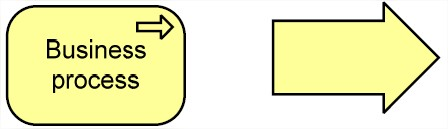
\includegraphics[width=35mm]{arquitectura/adm_lenguaje/imgs/business/BusinessProcess}          \\ \hline		
	Función de Negocio    		& \begin{tabular}[c]{p{7cm}@{}l@{}}Un elemento de comportamiento que agrupa el comportamiento basado en un conjunto de criterios elegidos (típicamente recursos comerciales requeridos y / o competencias).\end{tabular} & 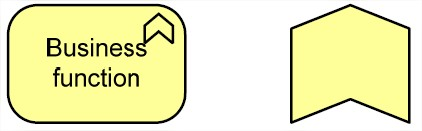
\includegraphics[width=35mm]{arquitectura/adm_lenguaje/imgs/business/BusinessFunction}          \\ \hline
	Interacción de Negocio    	& \begin{tabular}[c]{p{7cm}@{}l@{}}Un elemento de comportamiento que describe la comportamiento de una colaboración empresarial.\end{tabular} & 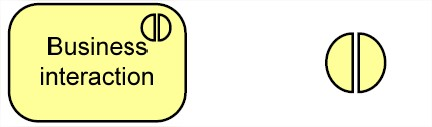
\includegraphics[width=35mm]{arquitectura/adm_lenguaje/imgs/business/BusinessInteraction}          \\ \hline
	Evento de Negocio    		& \begin{tabular}[c]{p{7cm}@{}l@{}}Algo que sucede (internamente o externamente) e influye en el comportamiento.\end{tabular} & 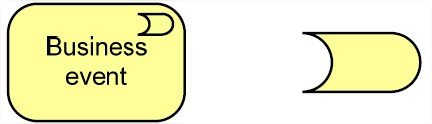
\includegraphics[width=35mm]{arquitectura/adm_lenguaje/imgs/business/BusinessEvent}          \\ \hline
	Servicio de Negocio    		& \begin{tabular}[c]{p{7cm}@{}l@{}}Un servicio que satisface una necesidad comercial de un cliente (interno o externo al organización).\end{tabular} & 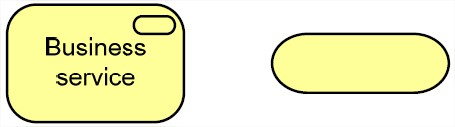
\includegraphics[width=35mm]{arquitectura/adm_lenguaje/imgs/business/BusinessService}          \\ \hline
	Representación    			& \begin{tabular}[c]{p{7cm}@{}l@{}}Una forma perceptible de la información llevado por un objeto comercial.\end{tabular} & 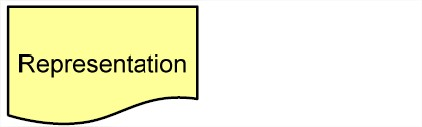
\includegraphics[width=35mm]{arquitectura/adm_lenguaje/imgs/business/Representation}          \\ \hline
	Meaning    					& \begin{tabular}[c]{p{7cm}@{}l@{}}El conocimiento o experiencia presente en un objeto comercial o su representación, dado un contexto particular.\end{tabular} & 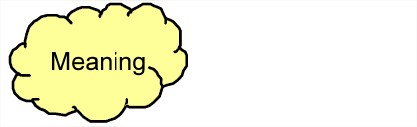
\includegraphics[width=35mm]{arquitectura/adm_lenguaje/imgs/business/Meaning}          \\ \hline
	Valor    					& \begin{tabular}[c]{p{7cm}@{}l@{}}El valor relativo, la utilidad o la importancia de un servicio o producto comercial.\end{tabular} & 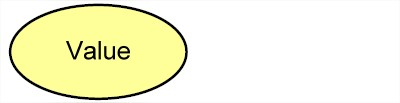
\includegraphics[width=35mm]{arquitectura/adm_lenguaje/imgs/business/Value}          \\ \hline
	Producto				    & \begin{tabular}[c]{p{7cm}@{}l@{}}Una colección coherente de servicios, acompañado de un contrato / conjunto de acuerdos, que se ofrece en su conjunto para (internos o externos) clientes.\end{tabular} & 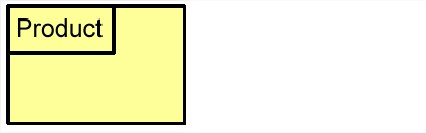
\includegraphics[width=35mm]{arquitectura/adm_lenguaje/imgs/business/Product}          \\ \hline
	Contrato				    & \begin{tabular}[c]{p{7cm}@{}l@{}}Una especificación formal o informal de acuerdo que especifica los derechos y obligaciones asociadas con un producto.\end{tabular} & 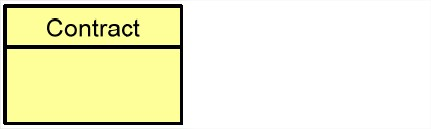
\includegraphics[width=35mm]{arquitectura/adm_lenguaje/imgs/business/Contract}          \\ \hline
\end{longtable}


\newpage

\subsection{Glosario Conceptos Capa de Aplicación}

\begin{longtable}[c]{|p{2.5cm}|l|c|}
	\caption{Conceptos Capa de Aplicación}
	\label{my-label}\\
	\hline
	\textbf{Concepto} 			& \textbf{Descripción}                                                                                                                                            & \textbf{Notación} \\ \hline
	\endhead
	%
	Componente de Aplicación	& \begin{tabular}[c]{p{7cm}@{}l@{}}Una parte modular, implementable y reemplazable de un sistema de software que encapsula su comportamiento y datos y los expone a través de un conjunto de interfaces.\end{tabular}                                                    & 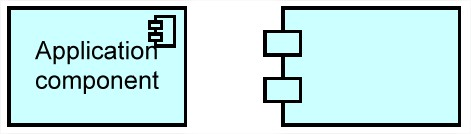
\includegraphics[width=35mm]{arquitectura/adm_lenguaje/imgs/application/ApplicationComponent}           \\ \hline
	Colaboración de Aplicaciones& \begin{tabular}[c]{p{7cm}@{}l@{}}Un agregado de dos o más componentes de aplicación que trabajan juntos para realizar un comportamiento colectivo.\end{tabular} & 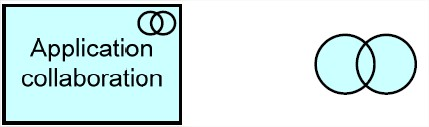
\includegraphics[width=35mm]{arquitectura/adm_lenguaje/imgs/application/ApplicationCollaboration}          \\ \hline
	Interfaz de Aplicación		& \begin{tabular}[c]{p{7cm}@{}l@{}}Un punto de acceso donde un servicio de aplicación está disponible para un usuario u otro componente de aplicación.\end{tabular} & 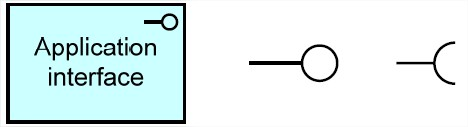
\includegraphics[width=35mm]{arquitectura/adm_lenguaje/imgs/application/ApplicationInterface}          \\ \hline
	Objeto de Datos				& \begin{tabular}[c]{p{7cm}@{}l@{}}Un elemento pasivo adecuado para el procesamiento automatizado..\end{tabular} & 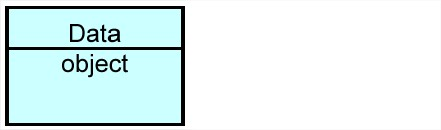
\includegraphics[width=35mm]{arquitectura/adm_lenguaje/imgs/application/DataObject}          \\ \hline
	Función de Aplicación		& \begin{tabular}[c]{p{7cm}@{}l@{}}Un elemento de comportamiento que agrupa el comportamiento automatizado que puede realizar un componente de la aplicación.\end{tabular} & 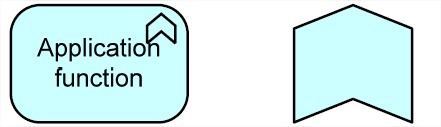
\includegraphics[width=35mm]{arquitectura/adm_lenguaje/imgs/application/ApplicationFunction}          \\ \hline
	Interacción de Aplicaciones	& \begin{tabular}[c]{p{7cm}@{}l@{}}Un elemento de comportamiento que describe el comportamiento de una colaboración de aplicaciones.\end{tabular} & 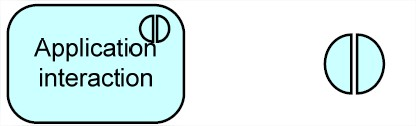
\includegraphics[width=35mm]{arquitectura/adm_lenguaje/imgs/application/ApplicationInteraction}          \\ \hline
	Servicio de Aplicación	   	& \begin{tabular}[c]{p{7cm}@{}l@{}}Un servicio que expone el comportamiento automatizado.\end{tabular} & 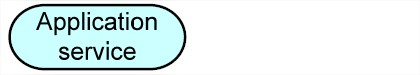
\includegraphics[width=35mm]{arquitectura/adm_lenguaje/imgs/application/ApplicationService}          \\ \hline
\end{longtable}

\newpage

\subsection{Glosario Conceptos Capa de Tecnología}


\begin{longtable}[c]{|p{2.55cm}|l|c|}
	\caption{Conceptos Capa de Tecnología}
	\label{my-label}\\
	\hline
	\textbf{Concepto} 			& \textbf{Descripción}                                                                                                                                            & \textbf{Notación} \\ \hline
	\endhead
	%
	Nodo  						& \begin{tabular}[c]{p{7cm}@{}l@{}}Un recurso computacional sobre el cual artefactos pueden ser almacenados o desplegados para ejecución.\end{tabular}                                                    & 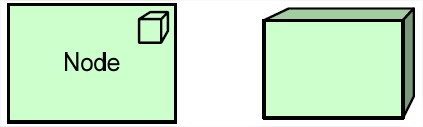
\includegraphics[width=35mm]{arquitectura/adm_lenguaje/imgs/technology/Node}           \\ \hline
	Dispositivo    				& \begin{tabular}[c]{p{7cm}@{}l@{}}Un recurso de hardware sobre el cual los artefactos pueden ser almacenado o desplegado para su ejecución.\end{tabular} & 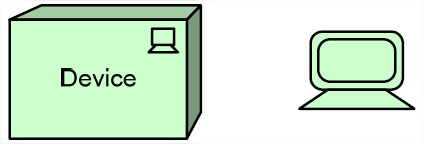
\includegraphics[width=35mm]{arquitectura/adm_lenguaje/imgs/technology/Device}          \\ \hline
	Network  					& \begin{tabular}[c]{p{7cm}@{}l@{}}Un medio de comunicación entre dos o más dispositivos..\end{tabular} & 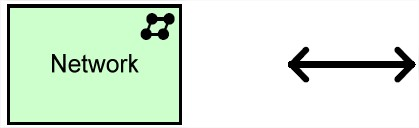
\includegraphics[width=35mm]{arquitectura/adm_lenguaje/imgs/technology/Network}          \\ \hline
	Ruta de comunicación		& \begin{tabular}[c]{p{7cm}@{}l@{}}Un enlace entre dos o más nodos, a través del cual estos nodos pueden intercambiar datos.\end{tabular} & 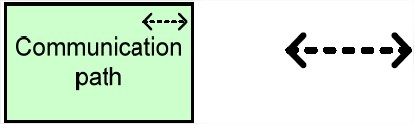
\includegraphics[width=35mm]{arquitectura/adm_lenguaje/imgs/technology/CommunicationPath}          \\ \hline
	Interfaz de Infraestructura	& \begin{tabular}[c]{p{7cm}@{}l@{}}Un punto de acceso al que otros nodos y componentes de la aplicación pueden acceder a servicios de infraestructura ofrecidos por un nodo.\end{tabular} & 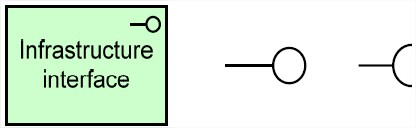
\includegraphics[width=35mm]{arquitectura/adm_lenguaje/imgs/technology/InfrastructureInterface}          \\ \hline
	Software del Sistema   		& \begin{tabular}[c]{p{7cm}@{}l@{}}Un entorno de software para tipos específicos de componentes y objetos que se implementan en él en forma de artefactos..\end{tabular} & 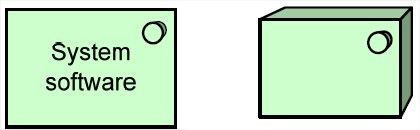
\includegraphics[width=35mm]{arquitectura/adm_lenguaje/imgs/technology/SystemSoftware}          \\ \hline
	Función de Infraestructura	& \begin{tabular}[c]{p{7cm}@{}l@{}}Un elemento de comportamiento que agrupa el comportamiento infraestructural que puede realizar un nodo.\end{tabular} & 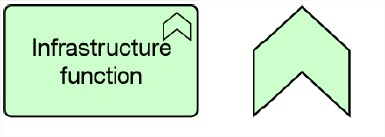
\includegraphics[width=35mm]{arquitectura/adm_lenguaje/imgs/technology/InfrastructureFunction}          \\ \hline		
	Servicio de Infraestructura	& \begin{tabular}[c]{p{7cm}@{}l@{}}Una unidad de funcionalidad externamente visible, proporcionada por uno o más nodos, expuesta a través de interfaces bien definidas y significativa para el entorno.\end{tabular} & 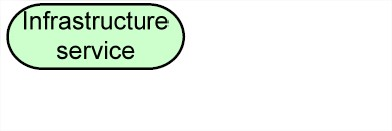
\includegraphics[width=35mm]{arquitectura/adm_lenguaje/imgs/technology/InfrastructureService}          \\ \hline
	Artefacto				   	& \begin{tabular}[c]{p{7cm}@{}l@{}}Una pieza física de datos que se utiliza o produce en un proceso de desarrollo de software, o mediante el despliegue y la operación de un sistema.\end{tabular} & 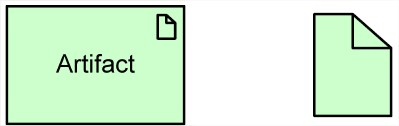
\includegraphics[width=35mm]{arquitectura/adm_lenguaje/imgs/technology/Artifact}          \\ \hline
\end{longtable}

\newpage

\subsection{Glosario Capa Motivacional}

\begin{longtable}[c]{|p{2.5cm}|l|c|}
	\caption{Conceptos Capa Motivacional}
	\label{my-label}\\
	\hline
	\textbf{Concepto} 			& \textbf{Descripción}                                                                                                                                            & \textbf{Notación} \\ \hline
	\endhead
	%
	Stakeholder					& \begin{tabular}[c]{p{7cm}@{}l@{}}El papel de un individuo, equipo u organización (o sus clases) que representa sus intereses o preocupaciones en relación con el resultado de la arquitectura.\end{tabular}                                                    & 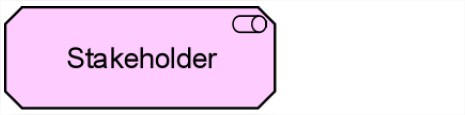
\includegraphics[width=35mm]{arquitectura/adm_lenguaje/imgs/motivational/Stakeholder}           \\ \hline
	Driver (Controlador)		& \begin{tabular}[c]{p{7cm}@{}l@{}}Algo que crea, motiva y alimenta el cambio en una organización.\end{tabular} & 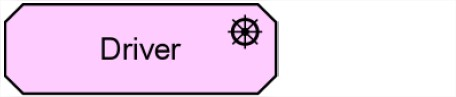
\includegraphics[width=35mm]{arquitectura/adm_lenguaje/imgs/motivational/Diver}          \\ \hline
	Assessment (Resultado)		& \begin{tabular}[c]{p{7cm}@{}l@{}}El resultado de algún análisis de algún controlador.\end{tabular} & 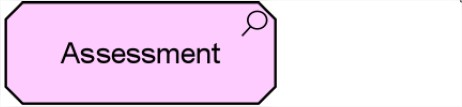
\includegraphics[width=35mm]{arquitectura/adm_lenguaje/imgs/motivational/Assessment}          \\ \hline
	Goal (Meta)					& \begin{tabular}[c]{p{7cm}@{}l@{}}Un estado final que una parte interesada intenta lograr.\end{tabular} & 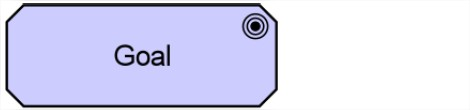
\includegraphics[width=35mm]{arquitectura/adm_lenguaje/imgs/motivational/Goal}          \\ \hline
	Requerimiento				& \begin{tabular}[c]{p{7cm}@{}l@{}}Una declaración de necesidad que debe ser realizada por un sistema.\end{tabular} & 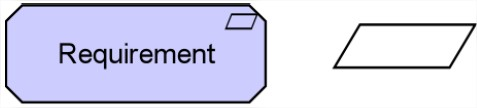
\includegraphics[width=35mm]{arquitectura/adm_lenguaje/imgs/motivational/Requirement}          \\ \hline
	Restricción					& \begin{tabular}[c]{p{7cm}@{}l@{}}Una restricción en la forma en que se realiza un sistema.\end{tabular} & 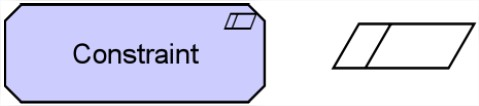
\includegraphics[width=35mm]{arquitectura/adm_lenguaje/imgs/motivational/Constraint}          \\ \hline
	Principle (Principio)	   	& \begin{tabular}[c]{p{7cm}@{}l@{}}Una propiedad normativa de todos los sistemas en un contexto dado, o la forma en que se realizan.\end{tabular} & 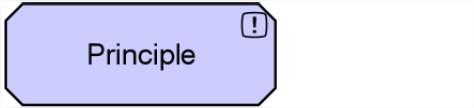
\includegraphics[width=35mm]{arquitectura/adm_lenguaje/imgs/motivational/Principle}          \\ \hline
\end{longtable}



\newpage

\subsection{Glosario Conceptos Capa de Implementación y Migración}

\begin{longtable}[c]{|p{2.5cm}|l|c|}
	\caption{Conceptos Capa de Implementación y Migración}
	\label{my-label}\\
	\hline
	\textbf{Concepto} 			& \textbf{Descripción}                                                                                                                                            & \textbf{Notación} \\ \hline
	\endhead
	%
	Paquete de Trabajo			& \begin{tabular}[c]{p{7cm}@{}l@{}}Una serie de acciones diseñadas para lograr un objetivo único dentro de un tiempo específico.\end{tabular}                                                    & 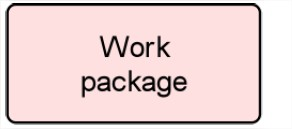
\includegraphics[width=35mm]{arquitectura/adm_lenguaje/imgs/implementacionMigration/WorkPackage}           \\ \hline
	Entregable					& \begin{tabular}[c]{p{7cm}@{}l@{}}Un resultado definido con precisión de un paquete de trabajo.\end{tabular} & 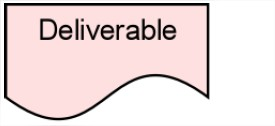
\includegraphics[width=35mm]{arquitectura/adm_lenguaje/imgs/implementacionMigration/Deliverable}          \\ \hline
	Plateau						& \begin{tabular}[c]{p{7cm}@{}l@{}}Un estado relativamente estable de la arquitectura que existe durante un período de tiempo limitado.\end{tabular} & 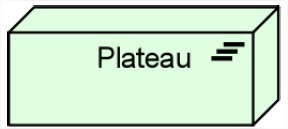
\includegraphics[width=35mm]{arquitectura/adm_lenguaje/imgs/implementacionMigration/Plateau}          \\ \hline
	Gap (Brecha)	   			& \begin{tabular}[c]{p{7cm}@{}l@{}}Un resultado de un análisis de brecha entre dos mesetas.\end{tabular} & 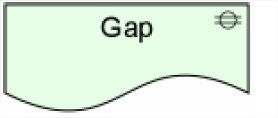
\includegraphics[width=35mm]{arquitectura/adm_lenguaje/imgs/implementacionMigration/Gap}          \\ \hline
\end{longtable}
